\documentclass[final]{beamer}


\usepackage[orientation=portrait,size=a0,scale=1.3]{beamerposter}


\usepackage[T1]{fontenc}
\usepackage[utf8]{inputenc}
\usepackage{lmodern}
\usepackage{tcolorbox}
\tcbuselibrary{skins}
\usepackage{amsmath,amssymb}
\usepackage{graphicx}
\graphicspath{{../figures/}}
\usepackage{ragged2e}
\usepackage[numbers,sort&compress]{natbib}
\usepackage{bibentry}
\usepackage{tikz}

\bibliographystyle{abbrv}

% --- strip all beamer chrome ---
\usetheme{default}
\setbeamertemplate{navigation symbols}{}
\setbeamertemplate{headline}{}
\setbeamertemplate{footline}{}

% --- colours ---
\definecolor{colKadcast}{HTML}{E63946}
\definecolor{colOPTIMUMP}{HTML}{E9C46A}
\definecolor{colKadRLNC}{HTML}{2A9D8F}
\definecolor{colAccent}{HTML}{1C2B3A}
\definecolor{colPanelBg}{HTML}{F7F7F2}
\definecolor{colPosterBg}{HTML}{EAEAEA}
\definecolor{colHeaderBg}{HTML}{1C2B3A}

% --- panel box style ---
\newtcolorbox{panel}[2]{
  enhanced,
  colback=colPanelBg, colframe=#2, colbacktitle=#2,
  coltitle=white, fonttitle=\bfseries\Large,
  title={#1}, boxrule=1.5pt, arc=4pt,
  top=10pt, bottom=10pt, left=12pt, right=12pt,
  toptitle=8pt, bottomtitle=8pt, lefttitle=12pt, righttitle=12pt
}

% --- font size helpers ---
\newcommand{\pbody}{\fontsize{21}{27}\selectfont}
\newcommand{\psmall}{\fontsize{17}{23}\selectfont}

% --- lengths (all in preamble) ---
\newlength{\colwidth}
\setlength{\colwidth}{0.3\paperwidth}
\newlength{\gutter}
\setlength{\gutter}{0.01\paperwidth}

%%%%%%%%%%%%%%%%%%%%%%%%%%%%%%%%%%%%%%%%%%%%%%%%%%%%%%%%%%%%
\begin{document}
\begin{frame}[t]

  % HEADER %%%%%%%%%%%%%%%%%%%%%%%%%%%%%%%%%%%%%%%%  
\begin{tcolorbox}[
  enhanced, colback=colHeaderBg, colframe=colHeaderBg,
  arc=0pt, boxrule=0pt,
  width=\paperwidth, left=18mm, right=18mm, top=12mm, bottom=12mm
  ]
  {\color{white}\fontsize{54}{64}\bfseries\selectfont
    A Comparative Analysis of Broadcasting Protocols in Blockchain Networks}\\[6pt]
  {\color{white}\fontsize{22}{30}\selectfont
    \textbf{Yojit Kumar (20231289)} \quad|\quad
    3rd year BS-MS, IISER Pune \quad|\quad
    \textbf{Supervisor: Dr Kalpesh Kapoor} \quad|\quad
    DS3613 Semester Project}
\end{tcolorbox}
%%%%%%%%%%%%%%%%%%%%%%%%%%%%%%%%%%%%%%%%%%%%%%%%%%%%%%%%%%%%


\vspace{7mm}


% THREE COLUMN %%%%%%%%%%%%%%%%%%%%%%%%%%%%%%%%%%%%%%%% 
\begin{columns}[T, totalwidth=0.95\paperwidth]

% COLUMN 1 %%%%%%%%%%%%%%%%%%%%%%%%%%%%%%%%%%%%%%%% 
\begin{column}{\colwidth}

% PANEL 1 %%%%%%%%%%%%%%%%%%%%%%%%%%%%%%%%%%%%%%%%   
\begin{panel}{1.\enspace Epidemic Modelling \& Gossip Protocols}{colAccent}
  \pbody\justifying

  My interest in this project originates from \textbf{epidemic modelling}, the study of how information, diseases, or disturbances propagate through a network of interacting agents. Gossip protocols borrow directly from this mathematics~\cite{demers1987}.
  Nodes occupy three states:
      
  \vspace{5pt}
      
  \begin{center}\pbody
    \textbf{Susceptible} $\;\longrightarrow\;$
    \textbf{Infected} $\;\longrightarrow\;$
    \textbf{Removed}
  \end{center}
  \begin{center}\psmall\color{gray}
    (uninformed) \hspace{28pt} (has block) \hspace{20pt} (done forwarding)
  \end{center}

  \vspace{7pt}

  The \textbf{SI model} corresponds to anti-entropy: every informed node continuously polls neighbours and pushes its data. The \textbf{SIR model} corresponds to rumour-mongering: a node stops spreading with probability $1/k$ after each round, modelling the decay of interest in already-known information~\cite{demers1987}.

  \vspace{7pt}
  In a gossip protocol, coverage grows exponentially at first then saturates; exactly the logistic curve of an epidemic. This gives us a principled way to study broadcast in decentralised systems: the same mathematical tools that model disease spread can bound how quickly information reaches all nodes.
\end{panel}
%%%%%%%%%%%%%%%%%%%%%%%%%%%%%%%%%%%%%%%%%%%%%%%%%%%%%%%%%%%%


\vspace{6mm}


% PANEL 2 %%%%%%%%%%%%%%%%%%%%%%%%%%%%%%%%%%%%%%%%   
\begin{panel}{2.\enspace Blockchains \& Broadcast Protocols}{colAccent}
  \pbody\justifying

  A blockchain is a distributed, append-only ledger that records transactions across a peer-to-peer network \textbf{without relying on a central authority}~\cite{nakamoto2008}. Because every node maintains a complete replica, every new block mined must be propagated to \emph{all} participants so that local copies remain synchronised~\cite{decker2013}. 

  \vspace{7pt}

  The mechanism that achieves this is the \textbf{broadcast protocol} --- the rules by which a message originating at one node is relayed until it reaches every other node~\cite{decker2013}. In Bitcoin's original implementation, a node announces a new block via an \textsc{inv} message (block hash only); neighbours without the block reply with \textsc{getdata} and receive the full block. This push-pull cycle repeats hop-by-hop across the network.

  \vspace{7pt}

  \textbf{Slow propagation is a security vulnerability.} The median time for a block to reach all Bitcoin nodes is 6.5~s, with 5\% still uninformed after 40~s. During this window a competing miner may produce a conflicting block, causing a fork ($\approx$1.7\% observed rate~\cite{decker2013}). An attacker holding as little as 49.1\% of hash power can mount a double-spend attack, a threshold that drops to $\approx$30\% under the threat of Selfish Mining~\cite{eyal2013}.
\end{panel}
%%%%%%%%%%%%%%%%%%%%%%%%%%%%%%%%%%%%%%%%%%%%%%%%%%%%%%%%%%%%


\vspace{6mm}


% PANEL 3 %%%%%%%%%%%%%%%%%%%%%%%%%%%%%%%%%%%%%%%%   
\begin{panel}{3.\enspace Measuring a Broadcast Protocol}{colAccent}
  \pbody\justifying

  A broadcast protocol must satisfy competing requirements simultaneously~\cite{decker2013,lai2025}. Three primary performance metrics are:

  \vspace{5pt}
   
  \begin{itemize}\setlength\itemsep{6pt}
    \item \textbf{Propagation latency} --- the time from block creation at the source to receipt at a target fraction of nodes (e.g.\ 50\%, 90\%, 99\%). Directly determines fork rate and consensus security.
    \item \textbf{Bandwidth overhead} --- the ratio of total messages transmitted across the network to the theoretical minimum needed for full coverage. Naive flooding achieves zero latency but at $\mathcal{O}{(N \times d)}$ message complexity~\cite{decker2013}.
    \item \textbf{Reliability \& fault tolerance} --- the fraction of nodes that successfully receive the block under node failures, packet loss, and adversarial behaviour. A protocol that is fast but fragile is worse than one that is slower but delivers with certainty.
  \end{itemize}

  \vspace{6pt}

  These three axes are in tension: reducing latency typically increases overhead; improving fault tolerance often increases both. Understanding this tradeoff is the central theme of this project~\cite{lai2025}. 
\end{panel}
%%%%%%%%%%%%%%%%%%%%%%%%%%%%%%%%%%%%%%%%%%%%%%%%%%%%%%%%%%%%


\vspace{6mm}


% PANEL 4 %%%%%%%%%%%%%%%%%%%%%%%%%%%%%%%%%%%%%%%%   
\begin{panel}{4.\enspace KadCast}{colKadcast}
  \pbody\justifying

  \begin{itemize}\setlength\itemsep{4pt}
    \item \textbf{Foundation:} Kadcast~\cite{kadcast2019} is built on Kademlia~\cite{maymounkov2002}, a DHT in which each node holds a random $L$-bit identifier and distance is the XOR metric: $d(x,y) = (x \oplus y)_{10}$.
    \item \textbf{Overlay Structure:} Each node organises known peers into $k$-buckets, where $B_i$ holds nodes at XOR distance $[2^i, 2^{i+1})$, enabling $O(\log N)$ traversal.
    \item \textbf{Mechanism:} A source selects $\beta$ nodes from each of its $L$ buckets and sends a \textsc{chunk} message with broadcast height $h$. Each receiver repeats this for buckets below $h$, recursively delegating subtree responsibility.
    \item This implicit spanning tree covers all $N$ nodes in $\Theta(\log N)$ steps with no central coordinator~\cite{kadcast2019}.
  \end{itemize}
  
  \vspace{5pt}
  
  \begin{center}
    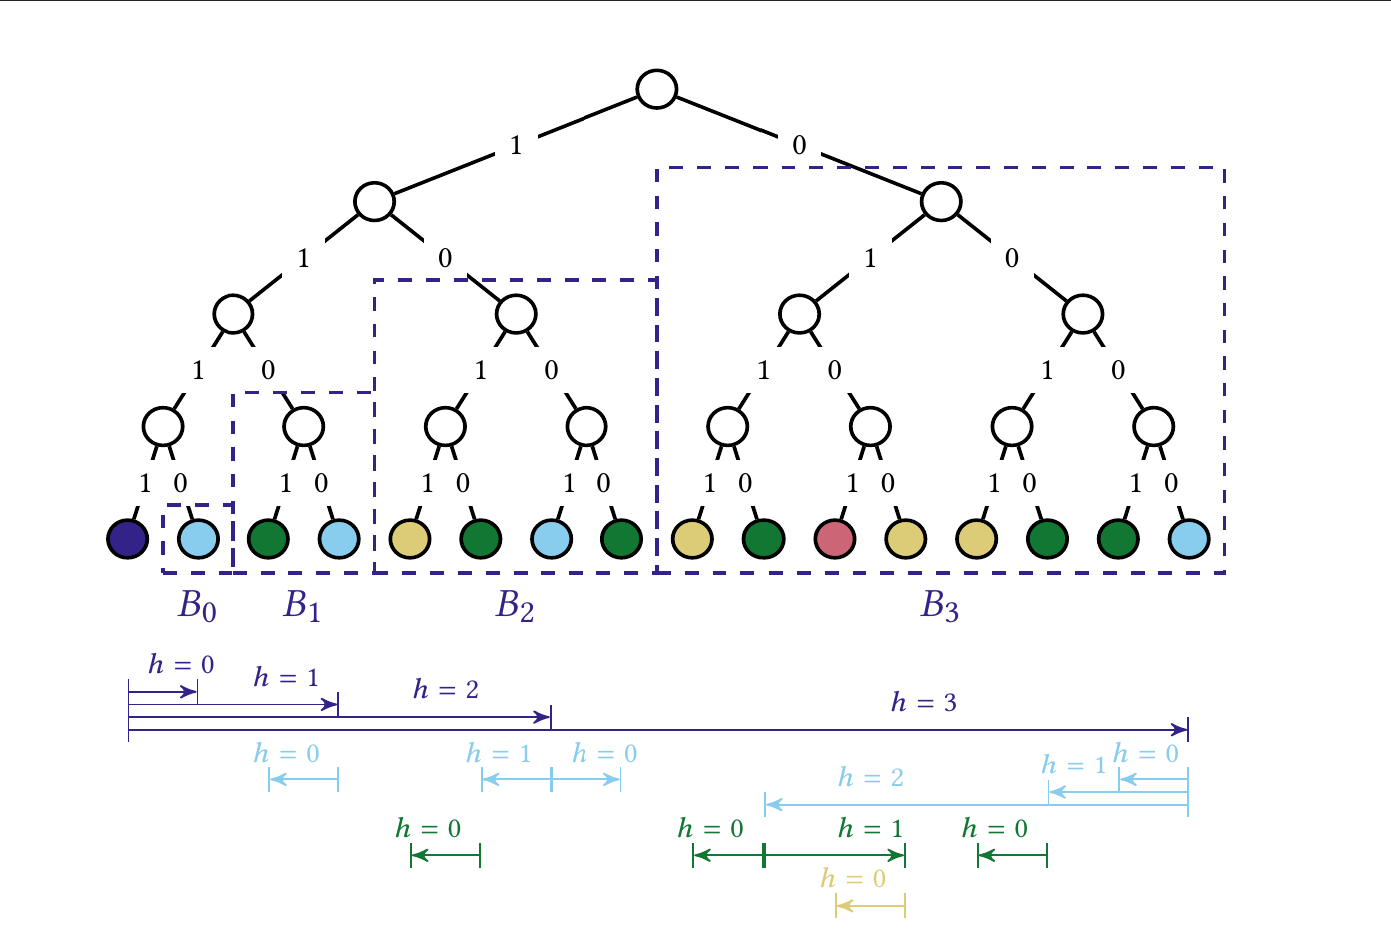
\includegraphics[width=0.5\linewidth]{kadcast.png}
  \end{center}

  \vspace{5pt}
  
  \textbf{Reliability:} (i)~$\beta > 1$ delegates per bucket; adversarial probability $(M/N)^\beta$ falls exponentially. (ii)~RaptorQ FEC: any $s$ of $n > s$ encoded symbols suffice for reconstruction~\cite{kadcast2019}.
  
  \vspace{5pt}
  
  \begin{itemize}\setlength\itemsep{4pt}
    \item \textbf{Performance:} In simulation ($N=500$, 1\,MB blocks), Kadcast reached 90\% coverage in 3784\,ms vs.\ 8461\,ms for vanilla gossip over 50\% faster~\cite{kadcast2019}.
    \item \textbf{Key limitation --- subtree starvation:} The XOR-tree structure means broadcast responsibility is delegated recursively down subtrees. A single relay node at height $h$ that fails or behaves maliciously can leave its \emph{entire} subtree without the block~\cite{kadcast2019}.
  \end{itemize}

\end{panel}
%%%%%%%%%%%%%%%%%%%%%%%%%%%%%%%%%%%%%%%%%%%%%%%%%%%%%%%%%%%%

\end{column}
%%%%%%%%%%%%%%%%%%%%%%%%%%%%%%%%%%%%%%%%%%%%%%%%%%%%%%%%%%%%


\hspace{\gutter}


% COLUMN 2 %%%%%%%%%%%%%%%%%%%%%%%%%%%%%%%%%%%%%%%%   
\begin{column}{\colwidth}

% PANEL 5 %%%%%%%%%%%%%%%%%%%%%%%%%%%%%%%%%%%%%%%%   
\begin{panel}{5.\enspace Optimump2p/RLNC Gossip}{colOPTIMUMP}
  \pbody\justifying
  
  \begin{itemize}\setlength\itemsep{4pt}
    \item \textbf{Purpose:} Optimump2p~\cite{optimump2p2025} is designed as a replacement for Gossipsub in Ethereum~2.0's libp2p stack, built on RLNC~\cite{ho2006}. Intermediate nodes forward \textbf{random linear combinations} of received packets over $\mathbb{F}_{2^q}$, it may achieve the min-cut capacity with error probability $\leq d/q$~\cite{ho2006}.
    \item \textbf{Mechanism:} The publisher divides the block into $k$ fragments, encodes into $p \cdot k$ coded shards, and pushes to all mesh neighbours. Each node accumulating $\geq r$ shards recodes and forwards. Any $k$ linearly independent shards suffice for Gaussian elimination decoding.
    \item \textbf{Haeupler's proof}~\cite{haeupler2010}: RLNC gossip achieves stopping time $\mathcal{O}{(k + T)}$ even in dynamically changing topologies.
    \item \textbf{Performace:} At 20 msg/s with 10\,MB blocks: Optimump2p held 2\,s latency and 99--100\% delivery; Gossipsub degraded to 4\,s and 80\% delivery~\cite{optimump2p2025}.
    \item \textbf{Key limitation --- topology blindness:} Optimump2p does not exploit network structure to reduce hop count. The stopping time $\mathcal{O}{(k + T)}$ is optimal \emph{given} $T$, but $T$ itself grows with the network diameter or inversely with the conductance $\lambda$ of the gossip mesh~\cite{haeupler2010}. On a poorly connected or geographically dispersed network, $T$ can be large, and RLNC does nothing to reduce it.
  \end{itemize}

\end{panel}
%%%%%%%%%%%%%%%%%%%%%%%%%%%%%%%%%%%%%%%%%%%%%%%%%%%%%%%%%%%%


\vspace{6mm}


% PANEL 6 %%%%%%%%%%%%%%%%%%%%%%%%%%%%%%%%%%%%%%%%   
\begin{panel}{6.\enspace A Hybrid Proposition}{colKadRLNC}
  \pbody\justifying

  \begin{itemize}\setlength\itemsep{4pt}
    \item Combines Kadcast's structural routing with RLNC's algebraic resilience to to address orthogonal failure modes.
    \item Kadcast's XOR tree ensures $\Theta(\log N)$ hop depth, bounding $T$.
    \item RLNC eliminates subtree starvation by letting downstream nodes \emph{pool partial coded shards} from multiple disrupted relay paths and collectively decode.
    \item \textbf{Design:} The source divides the block into $k$ fragments and encodes them into $n$ coded shards over $\mathbb{F}_{2^q}$ and selects one representative per Kademlia bucket as reciever.
    \item \textbf{Theoretical guarantee:} The broadcast executes on $G_{\mathrm{kad}}$, with diameter $O(\log N)$ and isoperimetric number $h = \Omega(1/\log N)$. Applying Haeupler's Lemma~6.5~\cite{haeupler2010} gives single-message stopping time $T = O(\log^2 N)$; Theorem~4.3 (perfect pipelining) then extends this to:
    \[
      T_{\mathrm{KadRLNC}} = O\!\left(k + \log^2 N\right)
    \]
  \end{itemize}
  The latency advantage over Optimump2p holds when $D_{\mathrm{gossip}} > \log N$.
\end{panel}
%%%%%%%%%%%%%%%%%%%%%%%%%%%%%%%%%%%%%%%%%%%%%%%%%%%%%%%%%%%%


\vspace{6mm}


% PANEL 7 %%%%%%%%%%%%%%%%%%%%%%%%%%%%%%%%%%%%%%%%   
\begin{panel}{7.\enspace Simulation Framework}{colAccent} 
  \pbody\justifying

  Protocols are evaluated in a custom \textbf{discrete-event simulator} (SimPy) on a 1000-node Kademlia overlay with 16-bit identifiers. Routing tables are precomputed with full global knowledge, capping each bucket at 10 randomly sampled peers.

  \vspace{5pt}

  \begin{itemize}\setlength\itemsep{4pt}
    \item \textbf{Bandwidth tiers:} 20\% infrastructure nodes at 1\,GB/s; 80\% consumer nodes at 50\,MB/s
    \item \textbf{Link latency:} sampled per-packet from LogNormal (median 50\,ms)
    \item \textbf{Contention:} shard transmissions serialised through a per-node uplink queue (SimPy Resource, capacity 1)
    \item \textbf{RLNC overhead:} fixed 5\,ms processing delay at recode and decode thresholds
    \item \textbf{Reproducible:} same graph instance and source node per protocol comparison; all stochastic elements seeded
  \end{itemize}
    
\end{panel}
%%%%%%%%%%%%%%%%%%%%%%%%%%%%%%%%%%%%%%%%%%%%%%%%%%%%%%%%%%%%


\vspace{6mm}


% PANEL 8 %%%%%%%%%%%%%%%%%%%%%%%%%%%%%%%%%%%%%%%%   
\begin{panel}{8.\enspace Experimental Design}{colAccent}
  \pbody\justifying

  \textbf{Experiment 1 --- Baseline Dissemination.} Single 1\,MB block, no competing traffic. Five broadcasts $\times$ ten seeds = 50 measurements per protocol. Isolates pure latency and coverage.

  \vspace{6pt}

  \textbf{Experiment 2 --- Publish Rate Stress Test.} Injection rates $\lambda \in \{1,2,4,8,16,32,64\}$ msg/s on shared uplink queues. Blocks tracked over a 5\,s window + 3\,s cooldown to avoid queue-relaxation artefacts. Measures delivery rate and latency under contention.

  \vspace{6pt}

  \textbf{Experiment 3 --- Payload Scaling.} Block sizes $\in \{128\,\text{KB},\ldots,4\,\text{MB}\}$, $k=32$ fixed (shard size scales proportionally). No contention. Isolates dissemination time and bandwidth overhead vs.\ payload.

  \vspace{7pt}

  \textbf{Metrics:} Time-to-Coverage CDF (50\%, 90\%, 99\%), Delivery Success Rate, Bandwidth Overhead (total shards / theoretical minimum).

\end{panel}
%%%%%%%%%%%%%%%%%%%%%%%%%%%%%%%%%%%%%%%%%%%%%%%%%%%%%%%%%%%%

\end{column}
%%%%%%%%%%%%%%%%%%%%%%%%%%%%%%%%%%%%%%%%%%%%%%%%%%%%%%%%%%%%


\hspace{\gutter}


% COLUMN 3 %%%%%%%%%%%%%%%%%%%%%%%%%%%%%%%%%%%%%%%%   
\begin{column}{\colwidth}

% PANEL 9 %%%%%%%%%%%%%%%%%%%%%%%%%%%%%%%%%%%%%%%%   
\begin{panel}{9.\enspace Results}{colAccent}
  \pbody

  \begin{center}
    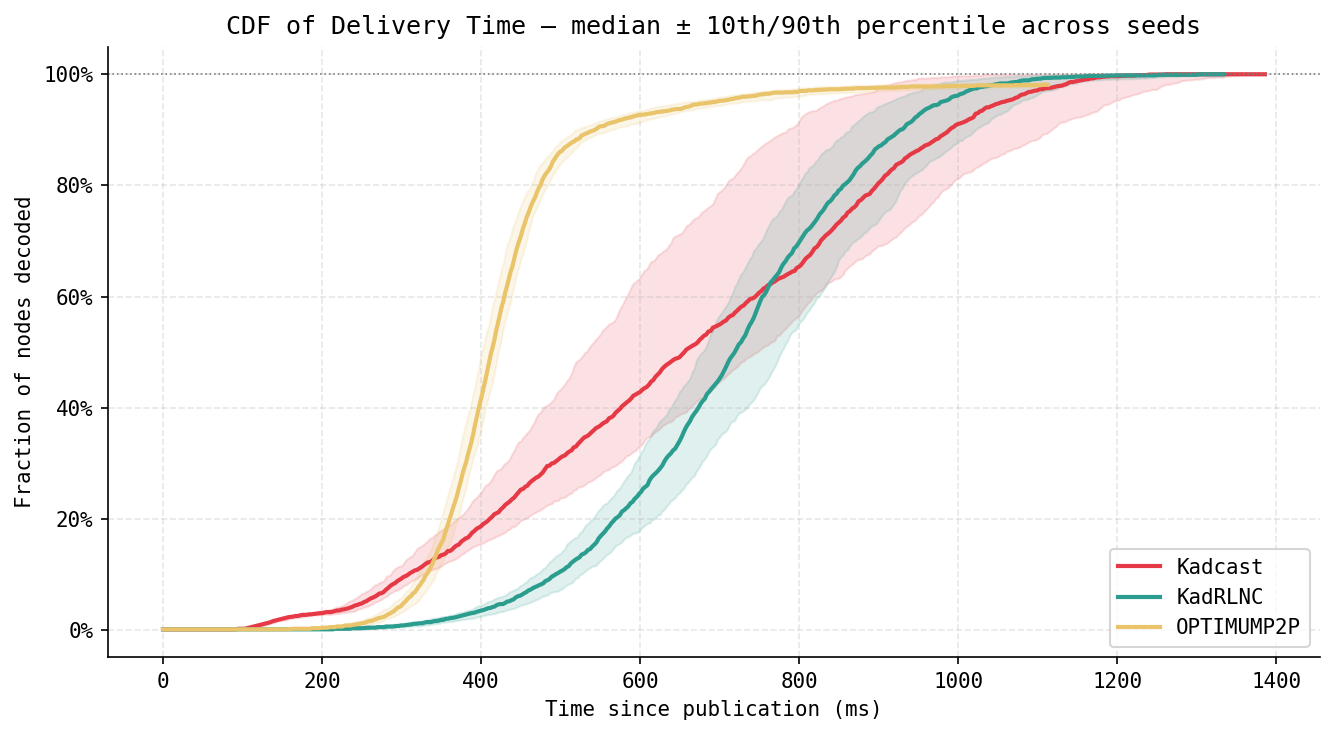
\includegraphics[width=\linewidth]{base/cdf_delivery.png}
  \end{center}
  
  \vspace{4mm}
  
  \begin{center}
    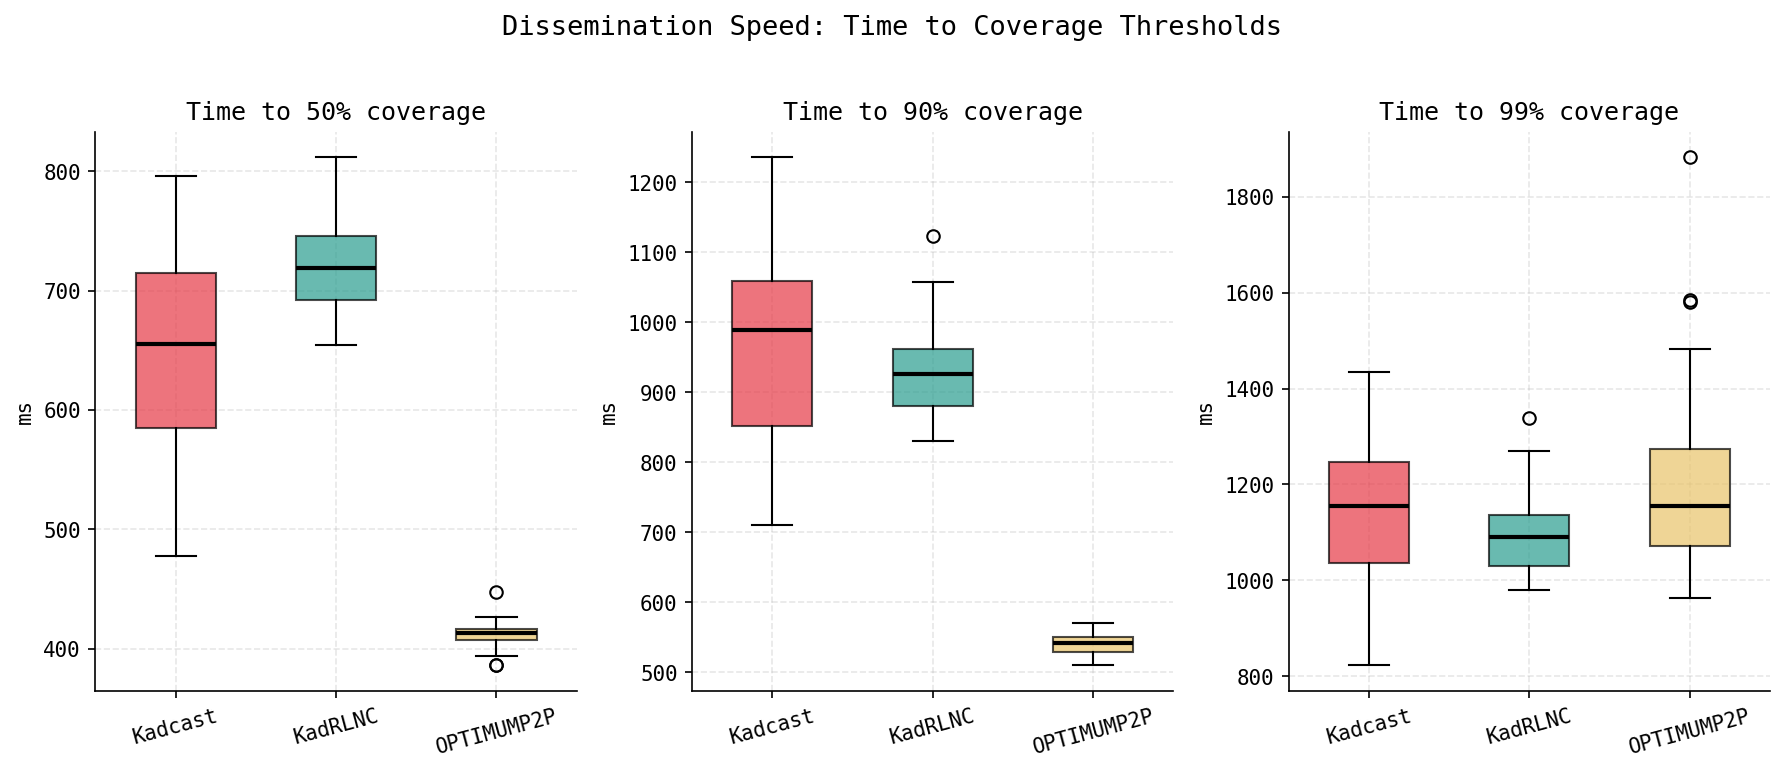
\includegraphics[width=\linewidth]{base/coverage_boxplots.png}
  \end{center}
  
  \vspace{4mm}
  
  \begin{center}
    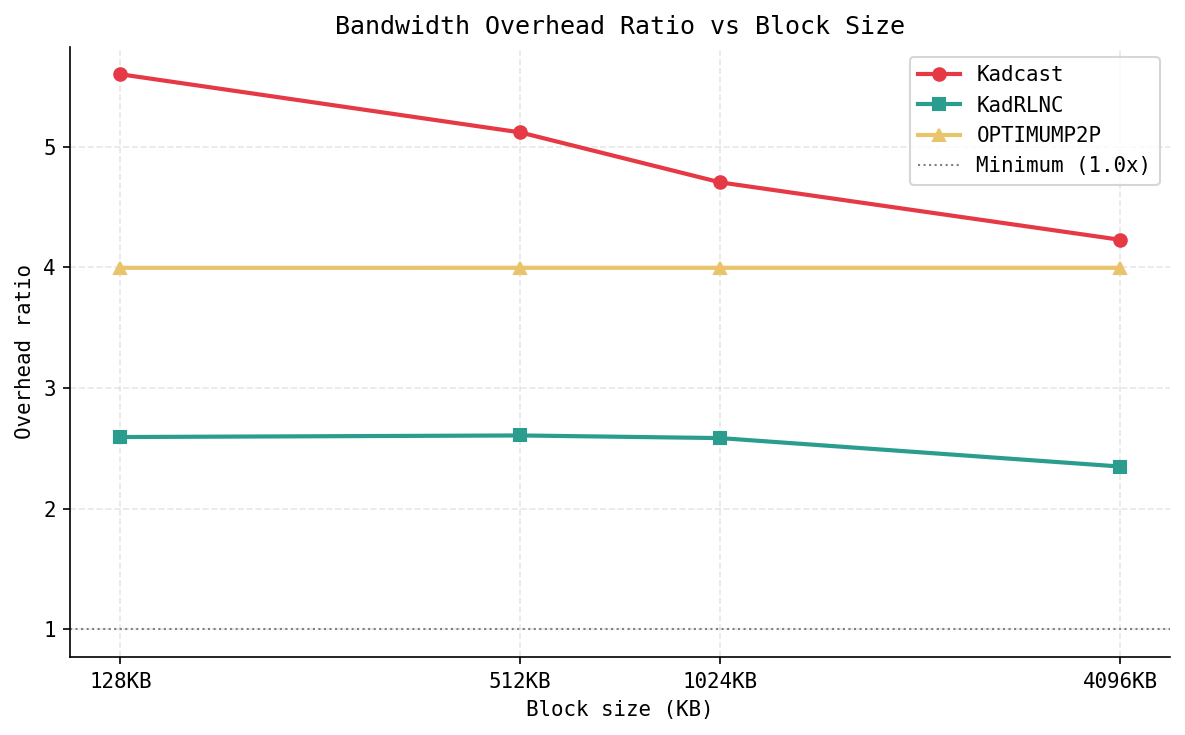
\includegraphics[width=\linewidth]{size/size_overhead.png}
  \end{center}
  
  \vspace{4mm}
  
  \begin{center}
    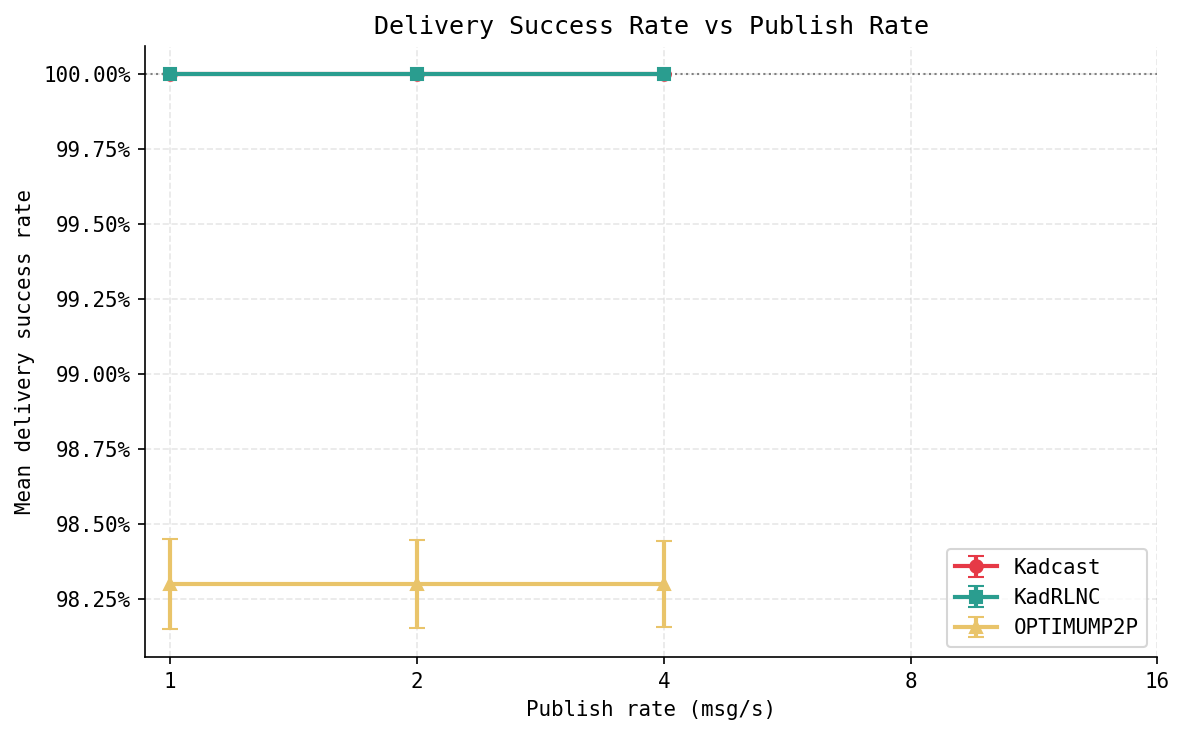
\includegraphics[width=\linewidth]{rate/rate_success.png}
  \end{center}

  \vspace{5pt}
  
  \psmall
  \textcolor{colKadcast}{\rule{14pt}{9pt}}~Kadcast \quad
  \textcolor{colOPTIMUMP}{\rule{14pt}{9pt}}~OPTIMUMP2P \quad
  \textcolor{colKadRLNC}{\rule{14pt}{9pt}}~KadRLNC
\end{panel}
%%%%%%%%%%%%%%%%%%%%%%%%%%%%%%%%%%%%%%%%%%%%%%%%%%%%%%%%%%%%


\vspace{6mm}


% PANEL 10 %%%%%%%%%%%%%%%%%%%%%%%%%%%%%%%%%%%%%%%%   
\begin{panel}{10.\enspace Conclusion \& Future Directions}{colKadRLNC}
  \pbody\justifying

  Kadcast exploits XOR geometry to achieve $\Theta(\log N)$ hop depth but its store-and-forward relay creates a hard subtree starvation vulnerability. Optimump2p achieves excellent delivery through RLNC-coded gossip but is topology-agnostic. KadRLNC was proposed to address both, with a theoretical stopping time of $O(k + \log^2 N)$.

  \vspace{7pt}
  
  The simulation results are more nuanced. OPTIMUMP2P was fastest at 50\% and 90\% coverage (median $\approx$410\,ms vs $\approx$720\,ms for KadRLNC). KadRLNC's genuine empirical advantage is \textbf{bandwidth efficiency} ($\approx$2.5$\times$ overhead vs $\approx$4$\times$ for OPTIMUMP2P and $\approx$5.5$\times$ for Kadcast) and graceful payload scaling. The latency gap is likely a scale artefact: at $N=1000$ with only 16 Kademlia buckets, the diameter advantage of $G_{\mathrm{kad}}$ is too small to overcome the fixed RLNC processing overhead.
  
  \vspace{7pt}
  
  \textbf{Future directions:}
  \begin{itemize}\setlength\itemsep{4pt}
    \item Evaluate KadRLNC at $N \geq 10{,}000$ where $D_{\mathrm{gossip}} \gg \log N$ is the realistic regime
    \item Introduce dynamic Byzantine node models
    \item Formally validate the combined bandwidth-latency parameter against established metrics
  \end{itemize}

\end{panel}
%%%%%%%%%%%%%%%%%%%%%%%%%%%%%%%%%%%%%%%%%%%%%%%%%%%%%%%%%%%%

\end{column}
%%%%%%%%%%%%%%%%%%%%%%%%%%%%%%%%%%%%%%%%%%%%%%%%%%%%%%%%%%%%

\end{columns}
%%%%%%%%%%%%%%%%%%%%%%%%%%%%%%%%%%%%%%%%%%%%%%%%%%%%%%%%%%%%


\vspace{8mm}


% FOOTER %%%%%%%%%%%%%%%%%%%%%%%%%%%%%%%%%%%%%%%%   
\begin{tcolorbox}[
  enhanced, colback=colHeaderBg, colframe=colHeaderBg,
  arc=0pt, boxrule=0pt,
  width=\paperwidth, left=18mm, right=18mm, top=10mm, bottom=10mm
  ]
  
  \phantom{\cite{decker2013,demers1987,eyal2013,haeupler2010,ho2006,kadcast2019,optimump2p2025,lai2025,nakamoto2008,li2021,liao2024,lin2022,maymounkov2002}}
  
  \begin{columns}[T]
    \begin{column}{0.78\linewidth}
      {\color{colPanelBg}\fontsize{27}{33}\bfseries\selectfont References}\\[5pt]
      {\color{white}\fontsize{23}{29}\selectfont
        [1]~Decker \& Wattenhofer. Information Propagation in the Bitcoin Network. \textit{IEEE P2P}, 2013. \quad
        [2]~Demers et al. Epidemic Algorithms for Replicated Database Maintenance. \textit{PODC}, 1987.\\[3pt]
        [3]~Eyal \& Sirer. Majority is not Enough. 2013. \quad
        [4]~Haeupler. Analyzing Network Coding Gossip Made Easy. \textit{STOC}, 2010. \quad
        [5]~Ho et al. A Random Linear Network Coding Approach to Multicast. \textit{IEEE Trans.\ Inf.\ Theory}, 2006.\\[3pt]
        [6]~Lai et al. Accelerating Block and Transaction Propagation. \textit{IEEE TNSE}, 2025. \quad
        [7]~Nakamoto. Bitcoin: A Peer-to-Peer Electronic Cash System. 2008.\\[3pt]
        [8]~Nicolaou et al. OPTIMUMP2P: Fast and Reliable Gossiping in P2P Networks. 2025. \quad
        [9]~Rohrer \& Tschorsch. Kadcast. \textit{ACM AFT}, 2019.
      }
      
      \nobibliography{references}
    \end{column}
  \end{columns}
\end{tcolorbox}
%%%%%%%%%%%%%%%%%%%%%%%%%%%%%%%%%%%%%%%%%%%%%%%%%%%%%%%%%%%%

\end{frame}
\end{document}
